\documentclass[12pt,fleqn,handout]{beamer}


\xdefinecolor{lavendar}{rgb}{0.8,0.6,1}
\xdefinecolor{olive}{cmyk}{0.64,0,0.95,0.4}
%\xdefinecolor{olive}{cmyk}{1,0,0,0}
\xdefinecolor{mag}{cmyk}{0.1,1,0,0.2}
\xdefinecolor{lblue}{rgb}{0,0,1.5}
\xdefinecolor{lred}{rgb}{1,0,0}
\xdefinecolor{mine}{cmyk}{1,0,0.2,0}
\xdefinecolor{bluel}{cmyk}{0.1,0,0.9,0.4}

\usepackage{amsmath,amssymb,dsfont,mathrsfs}
\usepackage{tikz,pgflibraryplotmarks}
\usepackage{multimedia}
\usepackage{wasysym}
\usepackage{rotating}
\usepackage{algorithm,algorithmic}
\usepackage{graphicx} % more modern
\usepackage{subfigure}
\usepackage{booktabs}

\usepackage{pgfplots}
\usepackage{verbatim}

\usepackage{setspace}
\newlength\iwidth
\newlength\iheight

\newcommand\makebeamertitle{\frame{\maketitle}}%
\graphicspath{{./images/}}
\setbeamertemplate{navigation symbols}{}
\addtobeamertemplate{navigation symbols}{}{%
    \usebeamerfont{footline}%
    \usebeamercolor[fg]{footline}%
	\insertshorttitle
    \;--
    \insertframenumber
}

\newcommand{\sectionstart}{
	\only<beamer>{
 	\begin{frame}% (fold)
 		\begin{centering}\Huge \insertsection \par\end{centering}
 	\end{frame}% frame the_application (end)
	}
 }


% make bibliography entries smaller
\usepackage{natbib}
\setbeamertemplate{bibliography item}{[\theenumiv]}
\renewcommand\bibfont{\scriptsize}
\setbeamertemplate{frametitle continuation}[from second]
\newcommand{\tcr}{\textcolor{red}}
\newcommand{\tcrd}{\textcolor{red}}
\newcommand{\tcb}{\textcolor{bluel}}
\newcommand{\tcm}{\textcolor{mag}}
\newcommand{\tcg}{\textcolor{olive}}

\newcommand{\R}{\mathbb{R}}
\newcommand{\C}{\mathbb{C}}

% bold lower-case for vectors
\newcommand{\bfa}{{\bf a}}
\newcommand{\bfb}{{\bf b}}
\newcommand{\bfc}{{\bf c}}
\newcommand{\bfs}{{\bf s}}
\newcommand{\bfm}{{\bf m}}
\newcommand{\bfd}{{\bf d}}
\newcommand{\bfe}{{\bf e}}
\newcommand{\bfu}{{\bf u}}
\newcommand{\bfy}{{\bf y}}
\newcommand{\bfx}{{\bf x}}
\newcommand{\bfh}{{\bf h}}
\newcommand{\bfw}{{\bf w}}
\newcommand{\bfv}{{\bf v}}
\newcommand{\bfr}{{\bf r}}
\newcommand{\bfz}{{\bf z}}
\newcommand{\bfp}{{\bf p}}


% bold upper-case for linear operators
\newcommand{\bfA}{{\bf A}}
\newcommand{\bfB}{{\bf B}}
\newcommand{\bfZ}{{\bf Z}}
\newcommand{\bfM}{{\bf M}}
\newcommand{\bfC}{{\bf C}}
\newcommand{\bfD}{{\bf D}}
\newcommand{\bfQ}{{\bf Q}}
\newcommand{\bfJ}{{\bf J}}
\newcommand{\bfG}{{\bf G}}
\newcommand{\bfI}{{\bf I}}
\newcommand{\bfP}{{\bf P}}
\newcommand{\bfK}{{\bf K}}
\newcommand{\bfY}{{\bf Y}}
\newcommand{\bfW}{{\bf W}}
\newcommand{\bfR}{{\bf R}}
\newcommand{\bfL}{{\bf L}}
\newcommand{\bfF}{{\bf F}}
\newcommand{\bfT}{{\bf T}}
\newcommand{\bfS}{{\bf S}}
\newcommand{\bfX}{{\bf X}}
\newcommand{\bfU}{{\bf U}}
\newcommand{\bfV}{{\bf V}}
\newcommand{\bfH}{{\bf H}}


\newcommand{\calF}{\mathcal{F}}



\newcommand{\hf}{{\frac 12}}
\newcommand{\bftheta}{{\boldsymbol \theta}}
\newcommand{\bfxi}{{\boldsymbol \xi}}

\newcommand{\bfLambda}{{\boldsymbol \Lambda}}
\newcommand{\bfSigma}{{\boldsymbol \Sigma}}
\newcommand{\bfepsilon}{{\boldsymbol \epsilon}}

\newcommand{\E}{\vec E}
\newcommand{\B}{\vec B}

\newcommand{\vu}{  {\vec {\bf u}}}

\newcommand{\grad}{  {\vec {\bf \nabla}}}

\newcommand{\lfrownie}{\textcolor{red}{\large{\frownie}}}
\newcommand{\lsmiley}{\textcolor{green}{\large{\smiley}}}

\newcommand{\curl}{\ensuremath{\nabla\times\,}}
\renewcommand{\div}{\nabla\cdot\,}
\newcommand{\divh}{\nabla_h\cdot\,}
\renewcommand{\grad}{\ensuremath{\nabla}}

\DeclareMathOperator*{\argmin}{arg\,min}
\date{}


\title{Introduction to Deep Neural Networks}
\subtitle{Numerical Methods for Deep Learning}

\begin{document}

\makebeamertitle

\section{Motivation} % (fold)
\label{sec:motivation}
\begin{frame}[fragile]\frametitle{Why Deep Networks?}

\begin{itemize}
\item Universal approximation theorem of NN suggests that we can approximate {\bf any} function by
two layers.
\item But - The width of the layer can be very large ${\cal O}(n\cdot n_f)$
\item
Deeper architectures can lead to more efficient descriptions of the problem.
\item
No real proof but lots of practical experience.
\end{itemize}


\end{frame}

\begin{frame}[fragile]\frametitle{Deep Neural Networks}

How deep is deep?

We will answer this question later ...

\bigskip
\pause

Until recently, the standard architecture was
\begin{eqnarray*}
\bfY_1 &=& \sigma(\bfK_0\bfY_0 + b_0) \\
\vdots & =&  \vdots \\
 \bfY_N &=& \sigma(\bfK_{N-1}  \bfY_{N-1}+ b_{N-1})
 \end{eqnarray*}

\bigskip
\pause

And use $\bfY_N$ to classify. This leads to the optimization problem
$$ 
\min_{\bfK_{0,\ldots,N-1},\bfb_{0,\ldots,N-1},\bfW} \ \ E\left(\bfW \bfY_N(\bfK_1,\ldots,\bfK_{N-1},b_1,\ldots, b_{N-1}) , \bfC^{\rm obs} \right)
 $$

\end{frame}

\begin{frame}[fragile]\frametitle{Example: The Alexnet~\cite{KrizhevskySutskeverHinton2012} for Image Classification}

\begin{columns}
	\column{.6\textwidth}
	\begin{itemize}
		\item Complex architectures 
		\item trained on multiple GPUs
		\item $\approx $ 60 million weights
	\end{itemize}	
	\column{.4\textwidth}
\begin{center}
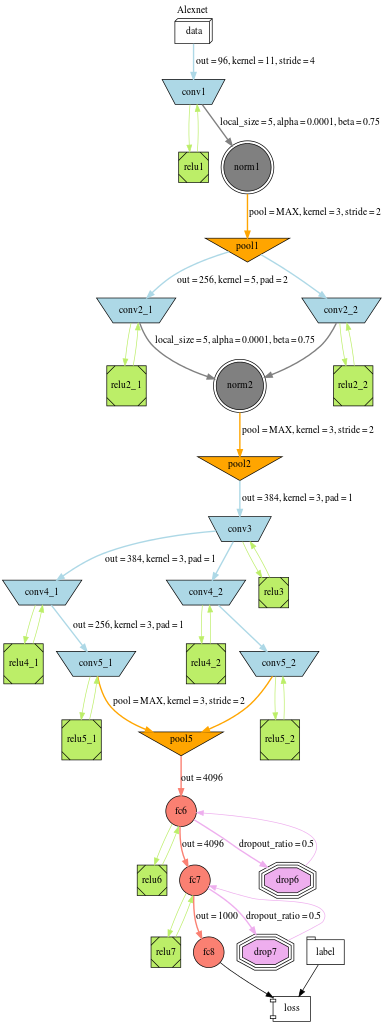
\includegraphics[width=2.9cm]{Alexnet-wikimedia}
\end{center}
\end{columns}




\end{frame}



\begin{frame}[fragile]\frametitle{Deep Neural Networks in Practice}

\begin{columns}
\column{.75\textwidth}
(Some) challenges:
\begin{itemize}
\item
Computational costs (architecture have millions or billions of parameters)
\item
difficult to design
\item
difficult to train (exploding/vanishing gradients)
\item
unpredictable performance
\end{itemize}

\bigskip
\invisible<beamer|1>{
In 2015, He et al.~\cite{he2016deep,he2016identity} came with a new architecture that solves many of the problems}
	
\column{.25\textwidth}
\invisible<beamer|1>{
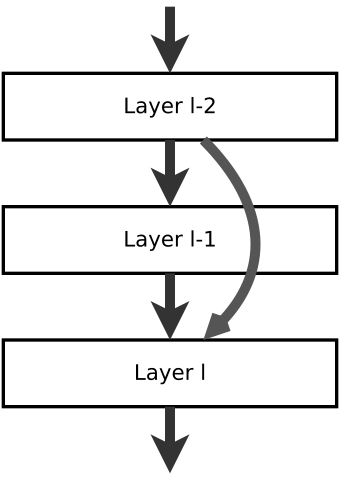
\includegraphics[width=30mm]{resnet-wikimedia}}
\end{columns}


\only<beamer|2>{}
\end{frame}




% section motivation (end)

\section{Residual Neural Networks} % (fold)
\label{sec:residual_neural_networks}

\begin{frame}[fragile]\frametitle{Simplified Residual Neural Network}

Residual Network

\bigskip

\begin{eqnarray*}
\bfY_1 &=& \bfY_0 + \sigma(\bfK_0\bfY_0 + b_0) \\
\vdots &=&  \vdots \\
 \bfY_N &=& \bfY_{N-1} + \sigma( \bfK_{N-1}\bfY_{N-1} + b_{N-1})
 \end{eqnarray*}

And use $\bfY_N$ to classify. This leads to the optimization problem
$$ 
\min_{\bfK_{0,\ldots,N-1},\bfb_{0,\ldots,N-1},\bfW} \ \ E\left(\bfW\bfY_N(\bfK_1,\ldots,\bfK_{N-1},b_1,\ldots, b_{N-1}), \bfC^{\rm obs} \right)
 $$

\bigskip
\begin{center}
	Leads to smoother objective function~\cite{LiEtAl2017}. 
	\end{center}

\end{frame}

\begin{frame}[fragile]\frametitle{Stability of Deep Residual Networks}

Why are ResNets more stable?

A small change
\begin{eqnarray*}
\bfY_1 &=& \bfY_0 + h \sigma(\bfK_0 \bfY_0  + b_0) \\
\vdots &=& \vdots \\
 \bfY_N &=& \bfY_{N-1} + h\sigma(\bfK_{N-1} \bfY_{N-1} + b_{N-1})
 \end{eqnarray*}

\bigskip
\pause 

This is nothing but a forward Euler discretization
of the  Ordinary Differential Equation (ODE)
$$ \dot{\bfY}(t) = \sigma(\bfK(t) \bfY(t)  + b(t)), \quad \quad \bfY(0) = \bfY_0 $$

We can understand the behavior by learning the dynamics of nonlinear ODEs~\cite{HaberRuthotto2017,E2017}.

\end{frame}

% section residual_neural_networks (end)

\section{Crash Course: ODE} % (fold)
\label{sec:crash_course_ode}
\begin{frame}[fragile]\frametitle{Crash Course on ODEs}

Given the ODE
$$ \dot{\bfy} = f(t,\bfy) $$
Assumptions:
\begin{enumerate}
	\item $f$ differentiable with Jacobian
$$ \bfJ(t,\bfy) = \left({\frac {\partial f}{\partial \bfy}}\right)^\top$$
	\item $\bfJ$ changes sufficiently slowly in time 
\end{enumerate} 


Then (see also~\cite{AscherPetzold1998,AscherGreif2011,Ascher2010})
\begin{itemize}
\item If $Re({\rm eig}(\bfJ)) > 0\quad \quad \rightarrow$\ Unstable
\item If $Re({\rm eig}(\bfJ)) < 0\quad \quad \rightarrow$\ Stable (converge to a stationary point)
\item If $Re({\rm eig}(\bfJ)) = 0\quad \quad \rightarrow$\ Stable, energy bounded
\end{itemize}


\end{frame}

\begin{frame}
	\frametitle{Stability of Residual Network}
	
	Assume forward propagation of single example $\bfy_0$
	$$ \dot{\bfy}(t) = \sigma(\bfK(t) \bfy(t) + b(t)), \quad \quad \bfy(0) = \bfy_0 $$
	
	\bigskip
	\pause
	
	The Jacobian is
	$$
	 \bfJ(t) = {\rm diag}\left(\sigma'(\bfK(t) \bfy(t) + b(t))\right) \bfK(t)
	$$
	Here, $\sigma'(x) \geq 0$ for $\tanh$, ReLU, \ldots
	
	\bigskip
	\pause
	
	Hence, problem is stable when
	\begin{enumerate}
		\item $\bfJ$ changes slowly in time
		\item $Re({\rm eig}\bfK(t)) \leq 0$ for every $t$
	\end{enumerate}
	
	\pause
	
	\begin{center}
		Remember that we  learn $\bfK$ $\leadsto$ ensure stability by regularization/constraints!
	\end{center}
	
	
\end{frame}


\begin{frame}[fragile]\frametitle{Residual Network as a Path Planning Problem}


\begin{center}
	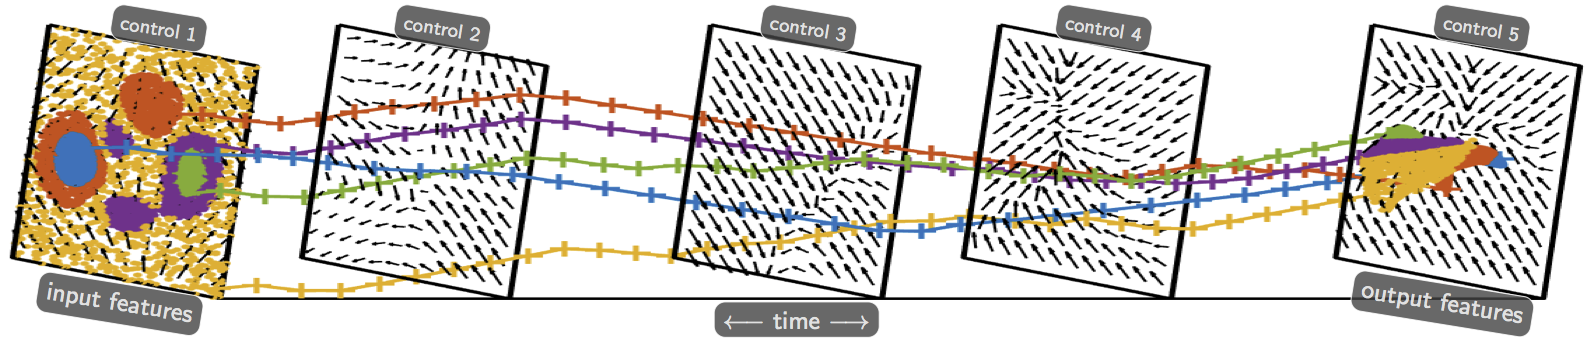
\includegraphics[width=\textwidth]{PathPlanning}
\end{center}

\bigskip
\pause

Forward propagation in residual network (continuous)
$$ \dot{\bfY}(t) = \sigma( \bfK(t) \bfY(t) + b(t)), \qquad \bfY(0) = \bfY_0 $$

The goal is to plan a path (via $\bfK$ and $b$) such that the initial data can be linearly separated

\bigskip
\pause
Question: What is a layer, what is depth?


\end{frame}



\begin{frame}[fragile]\frametitle{Stability: Continuous vs. Discrete}


Assume $\bfK$ is chosen so that the (continuous) forward propagation is stable
$$ \dot{\bfY}(t) = \sigma( \bfK \bfY(t)+ b(t)), \qquad \bfY(0) = \bfY_0 $$

And assume we use the forward Euler method to discretize
$$ \bfY_{j+1} = \bfY_{j} + h \sigma( \bfK_j \bfY_j + b_j) $$

Is the network stable?


\bigskip
\pause

Not always ...


\end{frame}


\begin{frame}[fragile]\frametitle{Stability: A Simple Example}

Look at the simplest possible forward propagation
$$ \dot{\bfY}(t) = \lambda\bfY(t) $$

And assume we use the forward Euler to discretize
$$ \bfY_{j+1} = \bfY_{j} + h \lambda \bfY_j = (1+h\lambda) \bfY_j$$

Then the method is stable only if
$$ |1+h\lambda| \le 1 $$

\bigskip

Not every network is stable! Time step size depends on our Jacobian

\end{frame}

\newcommand{\image}[1]{\includegraphics[width=35mm,trim=50 0 70 0,clip=true]{images/E10_Stability/#1}}
\newcommand{\rottext}[1]{\rotatebox{90}{\hbox to 40mm{\hss  #1\hss}}}
 \newcommand{\imageDiff}[1]{\includegraphics[width=35mm,trim=50 0 0 0,clip=true]{images/E10_Stability/#1}}
\begin{frame}
	\frametitle{Why you should care about stability - 1}
	
$$ 
\min_\theta \hf \|\bfY_N(\theta) - \bfC\|_F^2 \quad \quad \bfY_{j+1}(\theta)  = \bfY_j(\theta) + \frac{10}{N} \tanh \left( \bfK \bfY_j(\theta) \right)
 $$ 
where $\bfC = \bfY_{200}(1,1)$, $\bfY_0 \sim \mathcal{N}(0,1)$, and
$$
 \bfK(\theta) = \begin{pmatrix} -\theta_1-\theta_2 &           \theta_1  &  \theta_2 \\
\theta_2    &    -\theta_1-\theta_2 &        \theta_1 \\
       \theta_1 & \theta_2   &    -\theta_1-\theta_2 \end{pmatrix} 
	   $$       
\begin{center}
\begin{tabular}{cc}
	objective, $N=5$ & objective, $N=100$\\
\image{Phic} &
\image{Phif} 
\end{tabular}
\pause

\textbf{\tcr{Next: Compare different inputs $\sim$ generalization}}
	\end{center}       
\end{frame}
\begin{frame}
	\frametitle{Why you should care about stability - 2}
	
\begin{center}
\begin{tabular}{@{}c@{}c@{}c@{}c@{}}
	& objective, $\bfY_0^{\rm train}$ & objective, $\bfY_0^{\rm test}$ & abs. diff\\
	\rottext{unstable, $N=5$}
	& \image{Phic}
	& \image{Phict}
	& \imageDiff{Phic-Phict}\\[-8mm]
	\rottext{stable, $N=100$}
	& \image{Phif}
	& \image{Phift}
	& \imageDiff{Phif-Phift}
\end{tabular}	
\end{center}       
\end{frame}


\begin{frame}[fragile]\frametitle{Stability: A Non-Trivial Example}

Consider the antisymmetric kernel model
$$
			\bfK(t) = \bfK(t) - \bfK(t)^\top
$$
Here, $Re({\rm eig}(\bfJ)(t))= 0$ for all $\theta$.

\bigskip
\pause
			
Assume we use the forward Euler to discretize
$$ \bfY_{j+1} = \bfY_{j} + h \sigma( (\bfK_j-\bfK_j^\top) \bfY_j + b_j) $$
Tricky question: How to pick $h$ to ensure stability?

\pause

Answer: Impossible since eigenvalues of Jacobian are imaginary. Need other method than forward Euler.
\end{frame}

\begin{frame}[allowframebreaks]
	\frametitle{References}
\bibliographystyle{abbrv}
\bibliography{NumDNN}

\end{frame}

\end{document}
